%-----------------------------------------------------------------------------------------------------------------------------------------------%
%	The MIT License (MIT)
%
%	Copyright (c) 2015 Jan Küster
%
%	Permission is hereby granted, free of charge, to any person obtaining a copy
%	of this software and associated documentation files (the "Software"), to deal
%	in the Software without restriction, including without limitation the rights
%	to use, copy, modify, merge, publish, distribute, sublicense, and/or sell
%	copies of the Software, and to permit persons to whom the Software is
%	furnished to do so, subject to the following conditions:
%	
%	THE SOFTWARE IS PROVIDED "AS IS", WITHOUT WARRANTY OF ANY KIND, EXPRESS OR
%	IMPLIED, INCLUDING BUT NOT LIMITED TO THE WARRANTIES OF MERCHANTABILITY,
%	FITNESS FOR A PARTICULAR PURPOSE AND NONINFRINGEMENT. IN NO EVENT SHALL THE
%	AUTHORS OR COPYRIGHT HOLDERS BE LIABLE FOR ANY CLAIM, DAMAGES OR OTHER
%	LIABILITY, WHETHER IN AN ACTION OF CONTRACT, TORT OR OTHERWISE, ARISING FROM,
%	OUT OF OR IN CONNECTION WITH THE SOFTWARE OR THE USE OR OTHER DEALINGS IN
%	THE SOFTWARE.
%	
%
%-----------------------------------------------------------------------------------------------------------------------------------------------%


%============================================================================%
%
%	DOCUMENT DEFINITION
%
%============================================================================%

%we use article class because we want to fully customize the page and dont use a cv template
\documentclass[10pt,A4]{article}	


%----------------------------------------------------------------------------------------
%	ENCODING
%----------------------------------------------------------------------------------------

%we use utf8 since we want to build from any machine
\usepackage[utf8]{inputenc}		

%----------------------------------------------------------------------------------------
%	LOGIC
%----------------------------------------------------------------------------------------

% provides \isempty test
\usepackage{xifthen}

%----------------------------------------------------------------------------------------
%	FONT
%----------------------------------------------------------------------------------------
\usepackage{hyperref}%linkleme
% some tex-live fonts - choose your own

%\usepackage[defaultsans]{droidsans}
%\usepackage[default]{comfortaa}
%\usepackage{cmbright}
\usepackage[default]{raleway}
%\usepackage{fetamont}
%\usepackage[default]{gillius}
%\usepackage[light,math]{iwona}
%\usepackage[thin]{roboto} 

% set font default
\renewcommand*\familydefault{\sfdefault} 	
\usepackage[T1]{fontenc}

% more font size definitions
\usepackage{moresize}		


%----------------------------------------------------------------------------------------
%	PAGE LAYOUT  DEFINITIONS
%----------------------------------------------------------------------------------------

%debug page outer frames
%\usepackage{showframe}			


%define page styles using geometry
\usepackage[a4paper]{geometry}		

% for example, change the margins to 2 inches all round
\geometry{top=1.75cm, bottom=-.6cm, left=1.5cm, right=1.5cm} 	

%use customized header
\usepackage{fancyhdr}				
\pagestyle{fancy}

%less space between header and content
\setlength{\headheight}{-5pt}		


%customize entries left, center and right
%\lhead{}
%\chead{ \small{Jan Küster  $\cdot$ Consultant and Software Engineer $\cdot$  Bremen, Germany  $\cdot$  \textcolor{sectcol}{\textbf{info@jankuester.com}}  $\cdot$ +49 176 *** *** **}}
%\rhead{}


%indentation is zero
\setlength{\parindent}{0mm}

%----------------------------------------------------------------------------------------
%	TABLE /ARRAY DEFINITIONS
%---------------------------------------------------------------------------------------- 

%for layouting tables
\usepackage{multicol}			
\usepackage{multirow}

%extended aligning of tabular cells
\usepackage{array}

\newcolumntype{x}[1]{%
	>{\raggedleft\hspace{0pt}}p{#1}}%


%----------------------------------------------------------------------------------------
%	GRAPHICS DEFINITIONS
%------------------------------------- --------------------------------------------------- 

%for header image
\usepackage{graphicx}

%for floating figures
\usepackage{wrapfig}
\usepackage{float}
%\floatstyle{boxed} 
%\restylefloat{figure}

%for drawing graphics		
\usepackage{tikz}				
\usetikzlibrary{shapes, backgrounds,mindmap, trees}


%----------------------------------------------------------------------------------------
%	Color DEFINITIONS
%---------------------------------------------------------------------------------------- 
\usepackage{color}

%accent color
\definecolor{bgcol}{RGB}{0,0,0}
%dark background color
\definecolor{sectcol}{RGB}{0,0,140}

%light background / accent color
\definecolor{softcol}{RGB}{225,225,225}

%light background / accent color
\definecolor{darkcol}{RGB}{0,0,0}

%============================================================================%
%
%
%	DEFINITIONS
%
%
%============================================================================%

%----------------------------------------------------------------------------------------
% 	HEADER
%----------------------------------------------------------------------------------------

% remove top header line
\renewcommand{\headrulewidth}{0pt} 

%remove botttom header line
\renewcommand{\footrulewidth}{0pt}	  	

%remove pagenum
\renewcommand{\thepage}{}	

%remove section num		
\renewcommand{\thesection}{}			

%----------------------------------------------------------------------------------------
% 	ARROW GRAPHICS in Tikz
%----------------------------------------------------------------------------------------

% a six pointed arrow poiting to the left
\newcommand{\tzlarrow}{(0,0) -- (0.2,0) -- (0.3,0.2) -- (0.2,0.4) -- (0,0.4) -- (0.1,0.2) -- cycle;}	

% include the left arrow into a tikz picture
% param1: fill color
%
\newcommand{\larrow}[1]
{\begin{tikzpicture}[scale=0.58]
	 \filldraw[fill=#1!100,draw=#1!100!black]  \tzlarrow
 \end{tikzpicture}
}

% a six pointed arrow poiting to the right
\newcommand{\tzrarrow}{ (0,0.2) -- (0.1,0) -- (0.3,0) -- (0.2,0.2) -- (0.3,0.4) -- (0.1,0.4) -- cycle;}

% include the right arrow into a tikz picture
% param1: fill color
%
\newcommand{\rarrow}
{
\begin{tikzpicture}[scale=0.7]
	\filldraw[fill=sectcol!100,draw=sectcol!100!black] \tzrarrow
 \end{tikzpicture}
}



%----------------------------------------------------------------------------------------
%	custom sections
%----------------------------------------------------------------------------------------

% create a coloured box with arrow and title as cv section headline
% param 1: section title
%
\newcommand{\cvsection}[1]
{
\colorbox{bgcol}{\mystrut \makebox[1\linewidth][l]{
\larrow{sectcol} \hspace{-8pt} \larrow{sectcol} \hspace{-8pt} \larrow{sectcol} \textcolor{white}{\textbf{#1}}\hspace{4pt}
}}\\
}

%create a coloured arrow with title as cv meta section section
% param 1: meta section title
%
\newcommand{\metasection}[2]
{
\begin{tabular*}{1\textwidth}{p{2.7cm} p{11cm}}
\larrow{bgcol}	\normalsize{\textcolor{sectcol}{#1}}&#2\\[12pt]
\end{tabular*}
}

%----------------------------------------------------------------------------------------
%	 CV EVENT
%----------------------------------------------------------------------------------------

% creates a stretched box as cv entry headline followed by two paragraphs about 
% the work you did
% param 1:	event time i.e. 2014 or 2011-2014 etc.
% param 2:	event name (what did you do?)
% param 3:	institution (where did you work / study)
% param 4:	what was your position
% param 5:	some words about your contributions
%
\newcommand{\cvevent}[5]
{
\vspace{8pt}
	\begin{tabular*}{1\textwidth}{p{3.3cm} p{11.9cm} x{9.5cm}}
 \textcolor{bgcol}{#1}& \textbf{#2} & \vspace{3.5pt}\textcolor{sectcol}{#3}

	\end{tabular*}
\vspace{-2pt}
\textcolor{softcol}{\hrule}
\vspace{6pt}
	\begin{tabular*}{1\textwidth}{p{1.3cm} p{15.4cm}}
&		 \larrow{bgcol} #4\\[3pt]
	\end{tabular*}

}
\newcommand{\patent}[5]
{
	\vspace{8pt}
	\begin{tabular*}{1\textwidth}{p{1.3cm} p{11.9cm} x{9.5cm}}
		\textcolor{bgcol}{#1}& \textbf{#2} & \vspace{3.5pt}\textcolor{sectcol}{#3}
		
	\end{tabular*}
	\vspace{-2pt}
	\textcolor{softcol}{\hrule}
	\vspace{6pt}
	\begin{tabular*}{1\textwidth}{p{1.3cm} p{15.4cm}}
		&		 \larrow{bgcol} #4\\[3pt]
	\end{tabular*}
	
}
\newcommand{\cveventi}[5]
{
	\vspace{8pt}
	\begin{tabular*}{1\textwidth}{p{3.3cm} p{20.8cm} x{3.9cm}}
		\textcolor{bgcol}{#1}& \textbf{#2} & \vspace{2.5pt}\textcolor{sectcol}{#3}
		
	\end{tabular*}
	\vspace{-12pt}
	\textcolor{softcol}{\hrule}
	\vspace{6pt}
	\begin{tabular*}{1\textwidth}{p{1.3cm} p{15.4cm}}
		&		 \larrow{bgcol} #4\\[3pt]
		&          \larrow{bgcol} #5\\[3pt]
	\end{tabular*}
	
}


\newcommand{\cvevento}[3]
{
	\vspace{8pt}
	\begin{tabular*}{1\textwidth}{p{3.3cm} p{9.3cm} x{3.9cm}}
		\textcolor{bgcol}{#1}& \textbf{#2} & \vspace{2.5pt}\textcolor{sectcol}{#3}
		
	\end{tabular*}
	\vspace{-12pt}
	\textcolor{softcol}{\hrule}
}
% creates a stretched box as 
\newcommand{\cveventmeta}[2]
{
	\mbox{\mystrut \hspace{87pt}\textit{#1}}\\
	#2
}

%----------------------------------------------------------------------------------------
% CUSTOM STRUT FOR EMPTY BOXES
%----------------------------------------- -----------------------------------------------
\newcommand{\mystrut}{\rule[-.3\baselineskip]{0pt}{\baselineskip}}

%----------------------------------------------------------------------------------------
% CUSTOM LOREM IPSUM
%----------------------------------------------------------------------------------------
\newcommand{\lorem}
{Lorem ipsum dolor sit amet, consectetur adipiscing elit. Donec a diam lectus.}



%============================================================================%
%
%
%
%	DOCUMENT CONTENT
%
%
%
%============================================================================%
\begin{document}


%use our custom fancy header definitions
\pagestyle{fancy}	


%---------------------------------------------------------------------------------------
%	TITLE HEADLINE
%----------------------------------------------------------------------------------------
\vspace{-20.55pt}

% use this for multiple words like working titles etc.
%\hspace{-0.25\linewidth}\colorbox{bgcol}{\makebox[1.5\linewidth][c]{\hspace{46pt}\HUGE{\textcolor{white}{\textsc{Jan Küster}} } \textcolor{sectcol}{\rule[-1mm]{1mm}{0.9cm}} \parbox[b]{5cm}{   \large{ \textcolor{white}{{IT Consultant}}}\\
% \large{ \textcolor{white}{{Resume}}}}
%}}

% use this for single words, e.g. CV or RESUME etc.
\hspace{-0.25\linewidth}\colorbox{bgcol}{\makebox[1.5\linewidth][c]{\HUGE{\textcolor{white}{\textsc{LEVENT TÜZÜN}} } \HUGE{\textcolor{white}{\textsc{}} } }}


%----------------------------------------------------------------------------------------
%	HEADER IMAGE
%----------------------------------------------------------------------------------------
\vspace{10pt}
\begin{figure}[H]
\hspace{0.76\linewidth}
	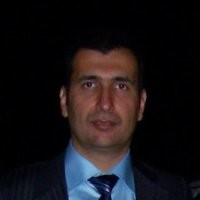
\includegraphics[width=0.25\linewidth]{image}	%trimming relative to image size!
\end{figure}

%---------------------------------------------------------------------------------------
%	QR CODE (optional)
%----------------------------------------------------------------------------------------
%\vspace{-136pt}
%\hspace{0.75\linewidth}
%
\includegraphics[width=103pt]{qrcode}
%\normalsize
%\vspace{88pt}

%---------------------------------------------------------------------------------------
%	META SECTION
%----------------------------------------------------------------------------------------

\vspace{-130pt}
\metasection{Tel:}{+90 (533) 462 88 84}
\metasection{E-posta:}{mail@gmail.com} 
\metasection{Adres:}{Adres}
\metasection{Doğum Tarihi:}{Tarih}
\metasection{Diller}{İngilizce}
\metasection{Hobiler}{Hobiler}


%---------------------------------------------------------------------------------------
%	SUMMARAY (optional)
%----------------------------------------------------------------------------------------

\cvsection{Hakkımda}\\
Ön Yazı
\\[-2pt]

%============================================================================%
%
%	CV SECTIONS AND EVENTS (MAIN CONTENT)
%
%============================================================================%

%---------------------------------------------------------------------------------------
%	EXPERIENCE
%----------------------------------------------------------------------------------------
\cvsection{Deneyimler}

%
\cvevent{2018-Devam Ediyor}{Otomotiv Sistem Tasarımı Grup Müdürü}{Vestel Elektronik}{Açıklama}

\cvevent{2001-2018}{STB Donanım Grup Müdürü}{Vestel Elektronik}{Açıklama}

\cvevent{1995-2001}{AR\&GE Müdürü}{Klemsan}{Açıklama}

\vspace{5pt}
%\textcolor{softcol}{\hrule}

%---------------------------------------------------------------------------------------
%	EDUCATION SECTION
%--------------------------------------------------------------------------------------
\cvsection{Akademik Hayatı}
%

\cvevento{2007-2009}{Bilkent Üniversitesi}{MBA}{}{}
\cvevento{1988-1992}{Selçuk Üniversitesi}{Elektronik Mühendisliği}

\vspace{5pt}

%\textcolor{softcol}{\hrule}

\cvsection{Yetenekler}

\textbf{Sektör Bilgisi}\\
Açıklama\\
\textbf{Araçlar ve Teknoloji}\\
C, C++, RTOS, Gömülü Linuz, Gömülü Yazılım, Gömülü Sistemler, IPTV \\
\textbf{Sosyal Yetenekler}\\
Mühendislik Yönetimi, Takım Yönetimi, Takım Liderliği\\
\textbf{Diğer Yetenekler}\\
H.264, DVB, MPEG, Mikroişlemciler, Zigbee, Akıllı Evler, Otomotiv Elektroniği, Elektronik Donanım Tasarımı\\
\vspace{5pt}

%-------------------------------------------------------------------------------------------------
%	ARTIFICIAL FOOTER (fancy footer cannot exceed linewidth) 
%--------------------------------------------------------------------------------------------------
%---------------------------------------------------------------------------------------
%Project SECTION
%--------------------------------------------------------------------------------------
\newpage
\cvsection{Patentler}

\patent{2011}{Dokunmatik Kontrol Özellikli Ekran}{}{Bir adet vericinin yanına konumlandırılmış olarak, kızıl ötesi vericileri aktive eden en az bir tarama aracı, alıcıların sinyal seviyesini tespit etmektedir. Ekran parametrelerinin ayarı için kullanılan ekran menüsünü de aktif hale getirmektedir. Engel ekrana yakın olduğunda ve engel ekranla temas halinde olduğunda tespit edilen sinyal seviyesine göre engelin pozisyonu tespit edilir.}{}

\patent{2010}{Görüntüleme Cihazları için Test Sistemi ve Yöntemi}{}{Televizyon, DVD, DVB gibi video çıkış cihazlarının ve cihazların tasarım aşamasında oluşabilecek makro blokaj, çerçeve atlama ve görüntü veri kaybı gibi belirli problemlerin tespiti ile ilgilidir.}{}
\patent{2010}{Daha Düşük Bekleme Gücü Tüketimi için Giriş Algılama Cihazı}{}{açıklama}{}
\patent{2009}{Bekleme Modunda Güç Tüketimini Azaltmak için Sistem ve Yöntem}{}{Elektronik cihaz tarafından normal çalışma koşulları altında tüketilen enerji, mevcut buluşa göre ana şebeke kaynağı tarafından sağlanır. Bekleme modu sırasında, yalnızca kullanıcı tarafından iletilen herhangi bir etkinleştirme sinyalini algılayacak olan elektronik bileşenler çalışır durumda tutulur.}{}
\patent{2007}{Taşınabilir Mikroislemci Kontrollü Para Sayma, Para Küpürü Tanıma/Ayırma ve Sahte Para Yakalama Cihazı}{}{Her türlü paranın sayımı, para küpürlerinin sayım esnasında tanınarak ayrılması ve sayım esnasında sahtelik kontrolü gereksinimlerini karşılamak amacıyla tasarlanmıştır.}{}

\patent{2000}{Tren Rayına Takılabilen Mikroişlemci Kontrollü Güç Kaynağı}{}{Doğru gerilim güç ihtiyacı duyulan her makine ve elektrik panosunda kullanılabilecek üzerinde merkezi mikroişlemci kontrolü ile fiziksel ve elektriksel korumaları olan "PushPull anahtarlamalı" modda çalışan yüksek verimli bir güç kaynağı ile ilgilidir.}{}
\patent{2000}{Klembus Haberleşme Protokolü Operatör Paneli.}{}{Özel protokol üzerinden haberleşen operatör panelidir.}{}
\vspace{5pt}
\cvsection{Yayınlar}

\patent{2012}{Dokunmatik Ekran OLED TV için Yeni Yöntem}{}{Açıklama}{}
\patent{2012}{Dokunmatik Özelikli AM-OLED Ekranlar için Alternatif Kontrol Yöntemi ve Testleri }{}{Ultraince tasarımlarda dokunmatik problemini görüntü kalitesini düşürmeden sağlayan yaklaşım sensörleri ile yapılması}\\
\patent{2011}{Parmak Yakınlık Tespiti Kullanarak Dokunmatik Ekran OLED TV Geliştirme Yöntemi}{}{Bilgi görüntüleme teknolojisinin gelişmesiyle birlikte son zamanlarda düz panel ekran (FPD) teknolojisi hız kazanmıştır. Organik ışık yayan diyot (OLED) teknolojisi, FPD arasında yapılan son araştırmadır. Daha önce hem dokunmatik ekranlı hem de aleve dayanıklı TV'ler Vestel firması tarafından LCD konseptinde tasarlanıyordu. Bu yazıda dokunmatik ekranlı OLED TV yapısının nasıl kurulduğu anlatılmaktadır.}\\
%\cvevent{20}{}{}\\
%\cvevent{20}{}{}
\vspace{5pt}
\newpage
\cvsection{Projeler}

\patent{2012}{Dokunmatik Ekran OLED TV için Yeni Yöntem}{}{Açıklama}{}
\patent{2012}{Dokunmatik Özelikli AM-OLED Ekranlar için Alternatif Kontrol Yöntemi ve Testleri }{}{Ultraince tasarımlarda dokunmatik problemini görüntü kalitesini düşürmeden sağlayan yaklaşım sensörleri ile yapılması}\\
\patent{2011}{Parmak Yakınlık Tespiti Kullanarak Dokunmatik Ekran OLED TV Geliştirme Yöntemi}{}{Bilgi görüntüleme teknolojisinin gelişmesiyle birlikte son zamanlarda düz panel ekran (FPD) teknolojisi hız kazanmıştır. Organik ışık yayan diyot (OLED) teknolojisi, FPD arasında yapılan son araştırmadır. Daha önce hem dokunmatik ekranlı hem de aleve dayanıklı TV'ler Vestel firması tarafından LCD konseptinde tasarlanıyordu. Bu yazıda dokunmatik ekranlı OLED TV yapısının nasıl kurulduğu anlatılmaktadır.}\\
%\cvevent{20}{}{}\\
%\cvevent{20}{}{}
\vspace{5pt}

\vspace{77pt}
%\vspace*{\fill}
%\hspace{-0.25\linewidth}\colorbox{bgcol}{\makebox[1.5\linewidth][c]{\mystrut \small \textcolor{white}{\href{https://www.linkedin.com/in/rabia-dogan-965439155/}{LinkedIn}} $\cdot$ \textcolor{white}{\href{https://github.com/rabikkk}{Github}}}}



%============================================================================%
%
%
%
%	DOCUMENT END
%
%
%
%============================================================================%
\end{document}
